\chapter{Spreading} % (fold)
\label{cha:spreading}

\section{Which model for news spreading?}

In order to choose a model for the spreading of news or ideas it's necessary to point out
what means in this field an infection, and to interpret the related quantities.
A person "infected'' by a news it's not a person just only reached by the news, but it's a person
who partecipates to the spreading by communicating to its neighbours and potentially infect them.
The decision to spread the information it's an individual choice, expressing the interest
of the person to the news, and indicates the presence of a personal threshold of reaction related to the news or ideas.
The threshold can also be influenced by the neighbourhood or the community membership.


In the epidemic models the coefficient $\beta$ represents the rate of trasmission of the infection and it is constant for the whole population, indicating the dependence on the properties of the pathogen.
In the news field $\beta$ can be interpreted as an intrinsic power of trasmission of the news.
This power of trasmission may be associated to the journalistic concept of \textit{newsworthiness},
which includes all the characteristics that make a fact a worthy news.
But the expanding phenomenon of \textit{fake news} shows that the speed of diffusion it's not only related to
the worthiness of an information. A recent paper published on Science \cite{Vosoughi_2018} shows how false news on Twitter spread 
``significantly farther, faster, deeper, and more broadly than the truth in all categories of information''.
The authors of the paper tried to explain the faster speed of diffusion of the false news by its novelty and the conveying
of strongest emotive reactions like surprise or disgust.
A news coverage is usually characterized also by a certain amount of time after which the news naturally ``dies'' out.
The SI and SIS epidemic models applied to free-scale networks predict asymptotically scenarios where there is always a finite 
fraction of infected nodes. From this point of view the SIR model may fit better to reality, predicting the vanishing of the news trasmission.
The coefficient $\mu$ of the epidemic models, likewise $\beta$, it's constant and in this case may represent the intrinsic property of a news to vanish, making the people stopping communicating about it. In summary:

\begin{itemize}
\item pathogen or agent: the news or information being spread.
\item infected node: a node that is communicating a news, for a certain period of time.
\item trasmission rate $\beta$: intrinsic power of trasmission of a news/information.
\item recover rate $\mu$: intrinsic rate related to a news at which the infected nodes stop communicating about it.
\item immunization: the node stops to communicate about the news definitely.
\item threshold: personal decision to communicate about the news or not, dependent or not on the neighbours decisions.
\end{itemize}


In this chapter we'll describe the results we obtained by applying the \textbf{SI}, \textbf{SIS}, \textbf{SIR},
and \textbf{Threshold} diffusion models both on the crawled data and on the synthetic graphs (Erdős–Rényi and
Barabási–Albert).

\section{SI model} % (fold)
\label{sec:si_model}


\begin{figure}[htbp]
  \centering
  \begin{subfigure}{0.45\textwidth}
    \resizebox{\textwidth}{!}{
      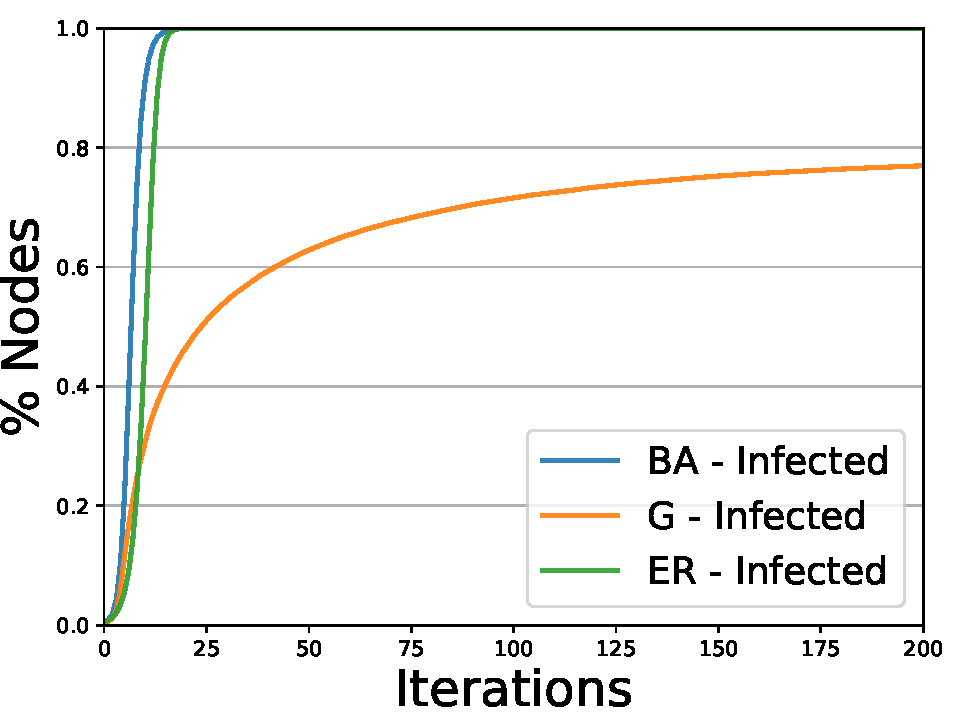
\includegraphics{images/spreading/si/trend_comparison_01.pdf}
    }
            \caption{Infection rate $\beta_0= 0.01$.}
            \label{fig:diff_si_1}
        \end{subfigure}
        \begin{subfigure}{0.45\textwidth}
            \resizebox{\textwidth}{!}{
              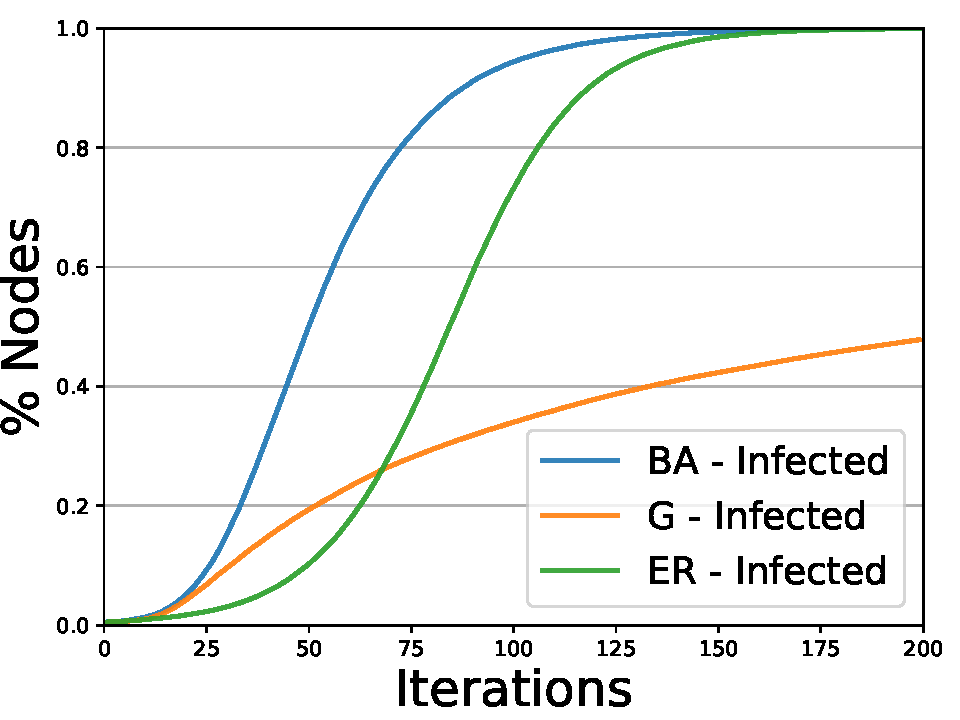
\includegraphics{images/spreading/si/trend_comparison_001.pdf}
            }
            \caption{Infection rate $\beta_1= \frac{\beta_0}{10} =  0.001$. }
            \label{fig:diff_si_2}
          \end{subfigure}
          \caption{Comparison of two trasmission rates in the SI model, for the original network $G$, the Erdos-Renyi $ER$ and the Barabasi-Albert $BA$.}
          \label{fig:diff_si}
     \end{figure}

For the \textbf{Susceptible-Infected} model we've started with a random $0.005\%$ of the total population ($3$ nodes)
    of each network being infected, representing the earliest sources of information.
    In Fig. \ref{fig:diff_si} we compare two different trasmission rates, with an order of magnitude of difference:
    $ \beta_0 =0.01$ for   $\beta_1 = 0.001$. The original network asymptotically reach the saturation regime only for the fraction of nodes
    in the strong connected component.


% section si_model (end)

\section{SIS model} % (fold)
\label{sec:sis_model}
    \begin{figure}[H]
        \centering
        \begin{subfigure}{0.3\textwidth}
            \resizebox{\textwidth}{!}{
                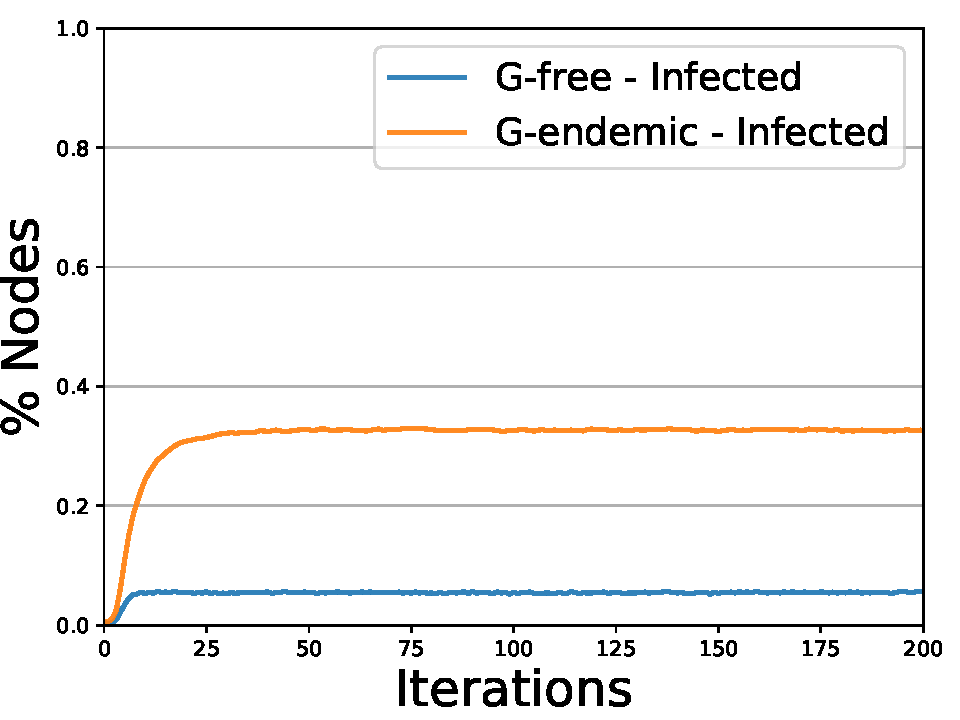
\includegraphics{images/spreading/sis/diffusion_G_comparison.pdf}
            }
            \caption{Original network}
            \label{diff_sis}
        \end{subfigure}
        \begin{subfigure}{0.3\textwidth}
            \resizebox{\textwidth}{!}{
                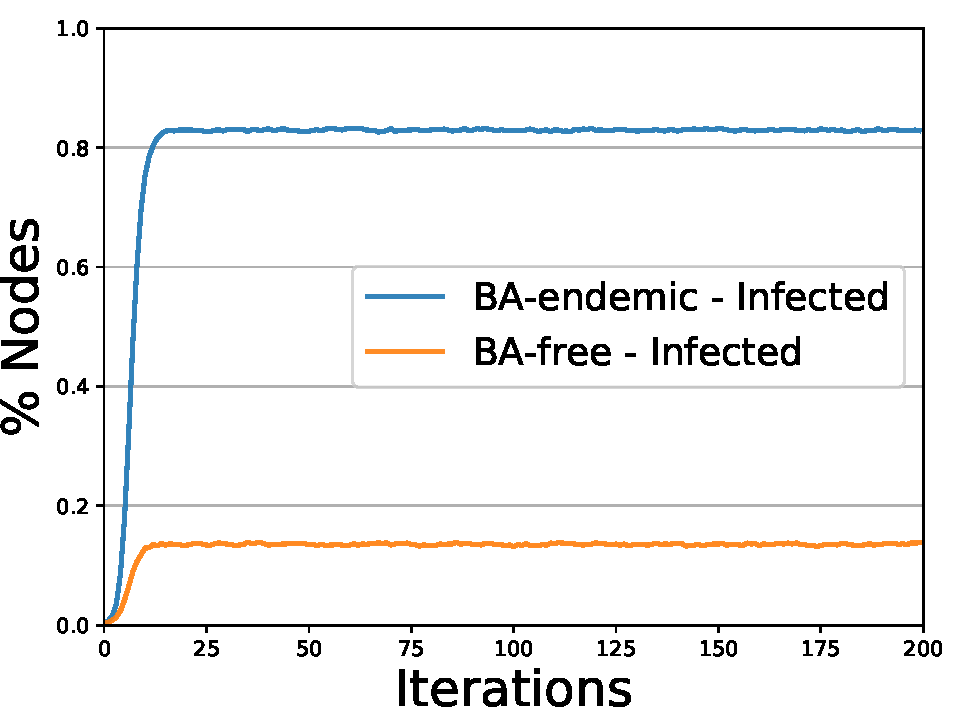
\includegraphics{images/spreading/sis/diffusion_BA_comparison.pdf}
            }
            \caption{Barabasi-Albert network}
            \label{diff_sis_er}
        \end{subfigure}
        \begin{subfigure}{0.3\textwidth}
            \resizebox{\textwidth}{!}{
                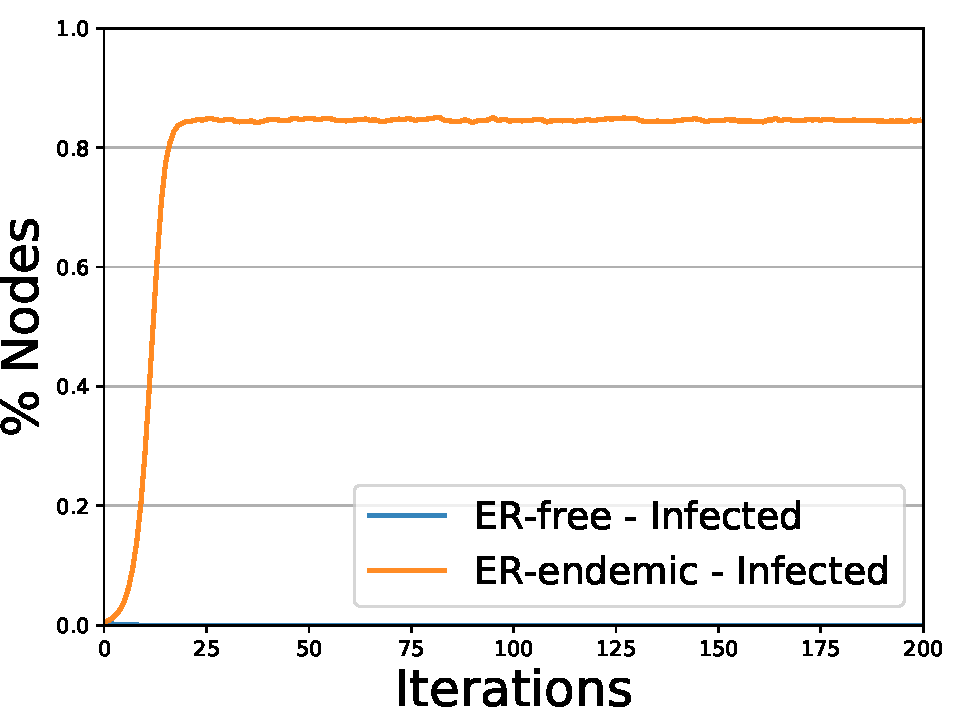
\includegraphics{images/spreading/sis/diffusion_ER_comparison.pdf}
            }
            \caption{Erdos-Renyi network}
            \label{diff_sis_ba}
        \end{subfigure}
        \caption{Comparison of the SIS model for the original network $G$, the Erdos-Renyi $ER$ and the Barabasi-Albert $BA$.}
        \label{fig:diff_sis_comparison}
      \end{figure}

      The introduction of the recovery rate $\mu$ in the \textbf{Susceptible-Infected-Susceptible} model for networks epidemics
      provides an epidemic threshold $\lambda_C$ for the spreading rate $\lambda$, dependent on the second order moment of the degree
      distribution $\langle k^2 \rangle$.
      For a random network the epidemic threshold given by Eq. \ref{eq:epidemic_threshold} is finite, and defines two possible asymptotically outcomes, an \textbf{endemic state} characterized by a finite fraction of infected individuals, and a completely \textbf{disease free} state.
      \begin{equation}
        \lambda_C(ER) = \frac{1}{\langle k \rangle +1 } \Rightarrow \lambda>\lambda_C:\: \text{epidemic state}
        \label{eq:epidemic_threshold}
      \end{equation}
      The free-scale networks are characterized by a diverging variance, which means the epidemic threshold tends to vanish, causing a finite fraction of infected individuals also for small $\lambda$. 
      We used the random network threshold to choose the recovery rate to simulate both the possible states. We observe in Fig. \ref{fig:diff_sis_comparison} how for the free-scale networks the infected fraction is always finite, below and above the epidemic threshold, while for the random network we observe also the disease free state.
      
% section sis_model (end)

\section{SIR model} % (fold){}
\label{sec:sir_model}
    The key characteristic of the \textbf{Susceptible-Infected-Recovered} model consists in the possibility
    of the individuals to recover from the disease and hence to be ``removed'' from the population instead of returning to the susceptible state.
    We tested this model either for the case in which $\mu$ is smaller than $\beta$ and the other way around.
    The different situations are represented in Fig. \ref{fig:diff_sir_total}, we observe the typical vanishing of the fraction of the infected nodes, after a steep initial rise similar to the one described by the SI model.

    \begin{figure}
        \begin{subfigure}{0.45\textwidth}
            \resizebox{\textwidth}{!}{
                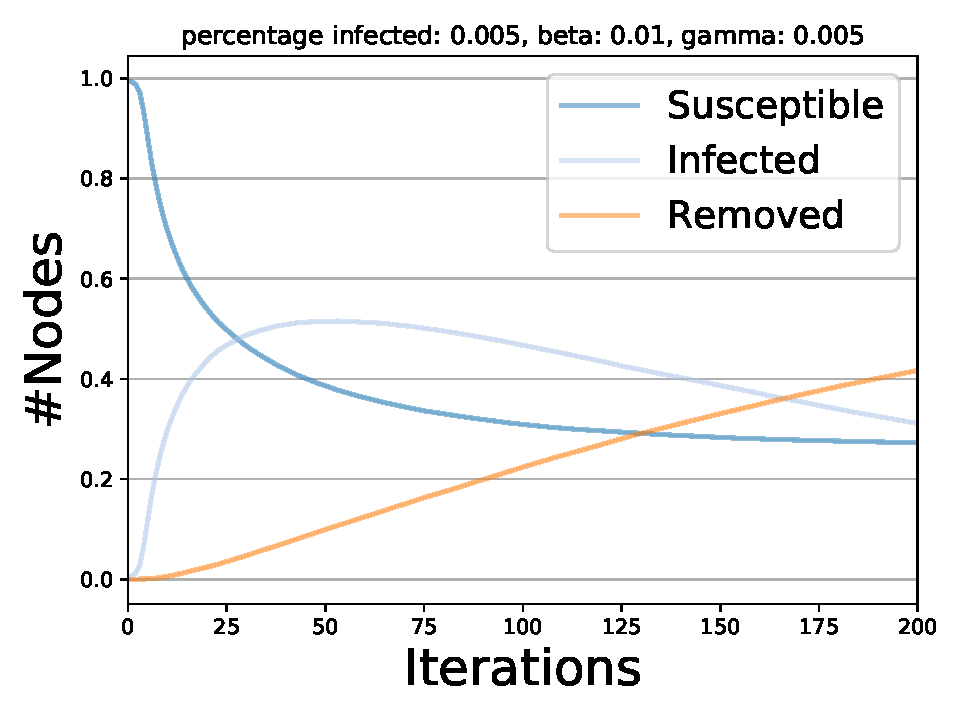
\includegraphics{images/spreading/sir/diffusion_smaller.pdf}
            }
            \caption{Original network}
            \label{diff_sir_smaller}
        \end{subfigure}
        \begin{subfigure}{0.45\textwidth}
            \resizebox{\textwidth}{!}{
                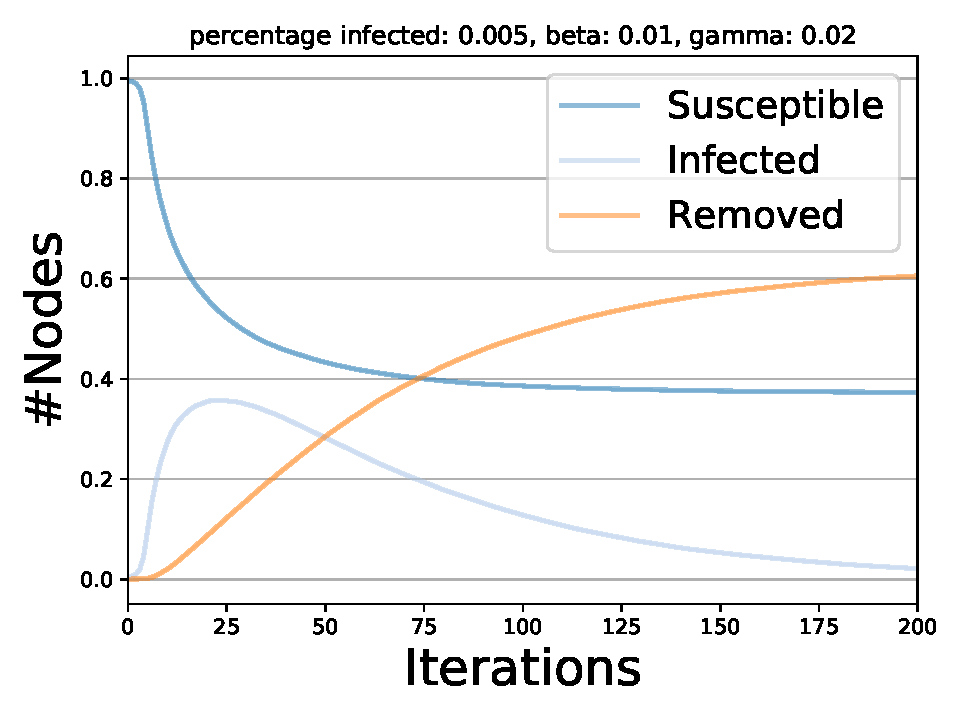
\includegraphics{images/spreading/sir/diffusion_greater.pdf}
            }
            \caption{Original network}
            \label{diff_sir_greater}
        \end{subfigure}
        \begin{subfigure}{0.45\textwidth}
            \resizebox{\textwidth}{!}{
                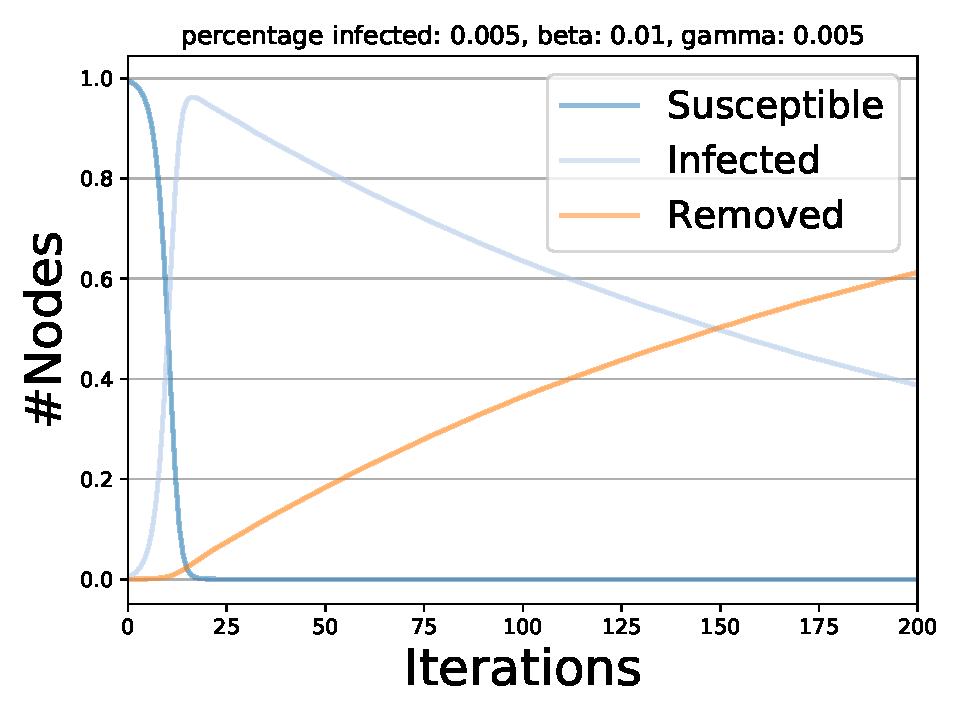
\includegraphics{images/spreading/sir/diffusion_er_smaller.pdf}
            }
            \caption{Erdos-Renyi network.}
            \label{diff_sir_er_smaller}
        \end{subfigure}
        \begin{subfigure}{0.45\textwidth}
            \resizebox{\textwidth}{!}{
                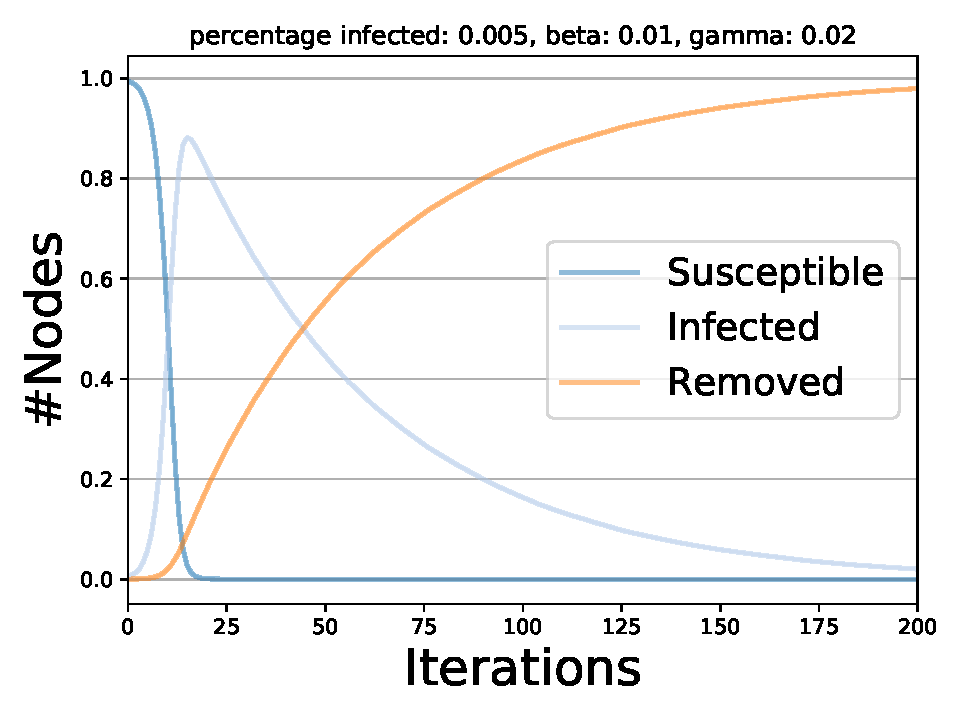
\includegraphics{images/spreading/sir/diffusion_er_greater.pdf}
            }
            \caption{Erdos-Renyi network.}
            \label{diff_sir_er_greater}
        \end{subfigure}
        \begin{subfigure}{0.45\textwidth}
            \resizebox{\textwidth}{!}{
                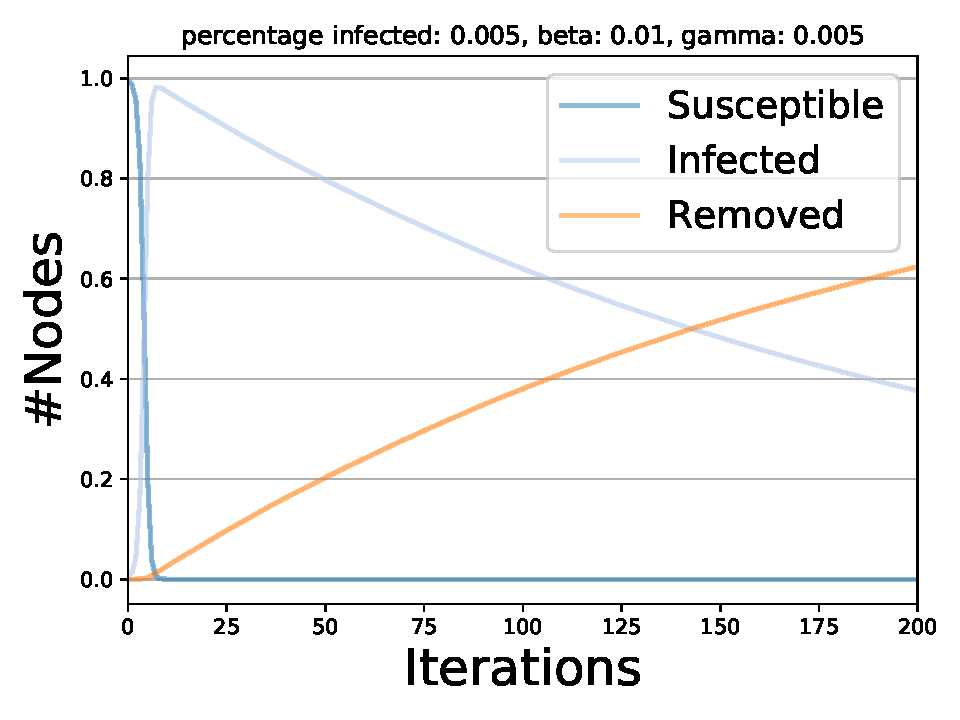
\includegraphics{images/spreading/sir/diffusion_ba_smaller.pdf}
            }
            \caption{Barabasi-Albert network.}
            \label{diff_sir_ba_smaller}
        \end{subfigure}
        \begin{subfigure}{0.45\textwidth}
            \resizebox{\textwidth}{!}{
                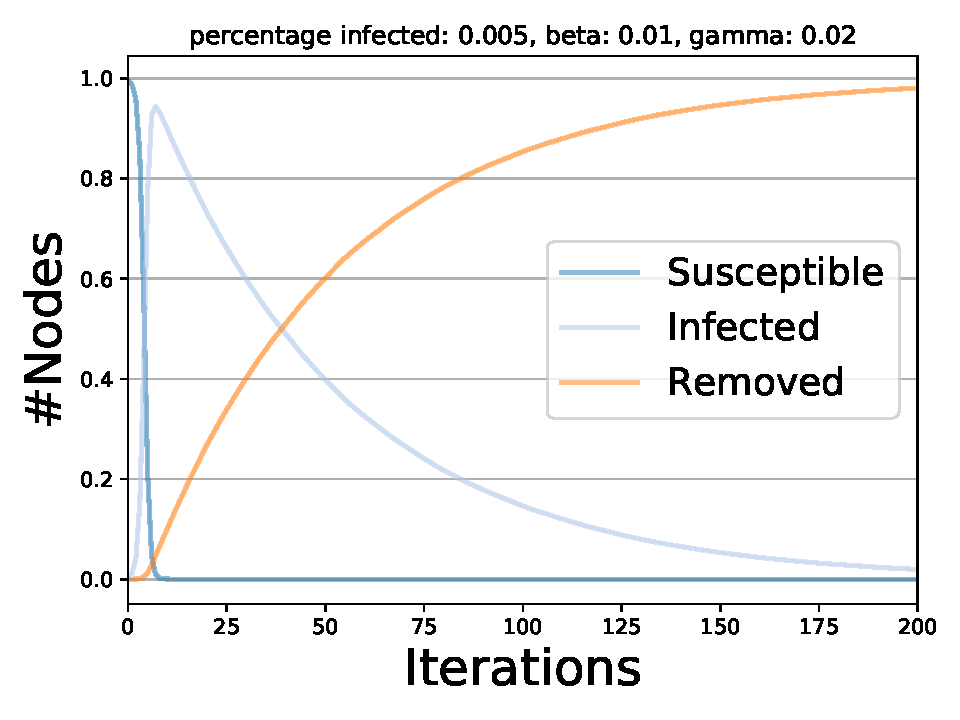
\includegraphics{images/spreading/sir/diffusion_ba_greater.pdf}
              }
            \caption{Barabasi-Albert network.}
            \label{diff_sir_ba_greater}
        \end{subfigure}
        \caption{SIR model applied to the networks, with two different $\lambda$ values.}
        \label{fig:diff_sir_total}
    \end{figure}

% section sir_model (end)

\section{Threshold model} % (fold)
\label{sec:threshold_model}

    In order to test the \textbf{Threshold model} we've chosen a threshold $\tau$ equal to $0.10$. The
    diffusion of the infection for this model is represented in Figure \ref{diff_thr_total}. As we can see, for the
    original network we have that almost all the nodes become infected within the first $20$ model's iterations,
    due to the fact that the value chosen for the threshold results sufficient for the spreading of the
    infection. If we change the threshold's value, this time using a value of $0.20$, we can observe that the
    original network become immune to the infection, thanks to its internal structure. We can observe
    the same immunity in the Erdős–Rényi and Barabási–Albert network for the original threshold's value.



    \begin{figure}[htbp]
        \begin{subfigure}{0.45\textwidth}
          \resizebox{\textwidth}{!}{
            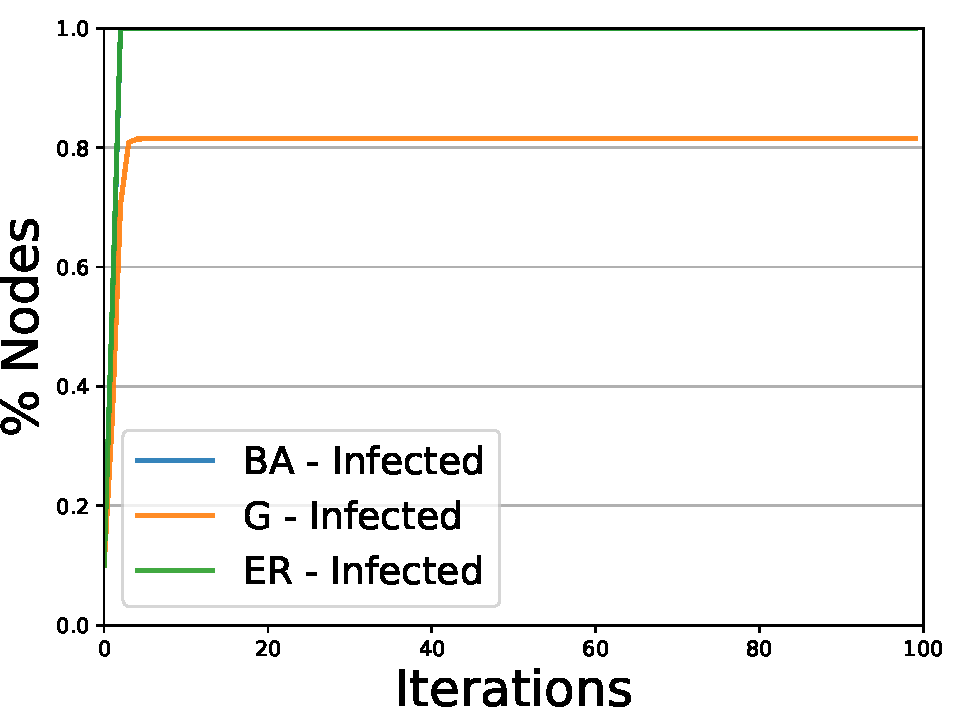
\includegraphics{images/spreading/threshold/trend_comparison_infection.pdf}
            }
            \caption{Endemic state with lower threshold, $\tau=0.1$}
        \end{subfigure}
        \begin{subfigure}{0.45\textwidth}
            \resizebox{\textwidth}{!}{
              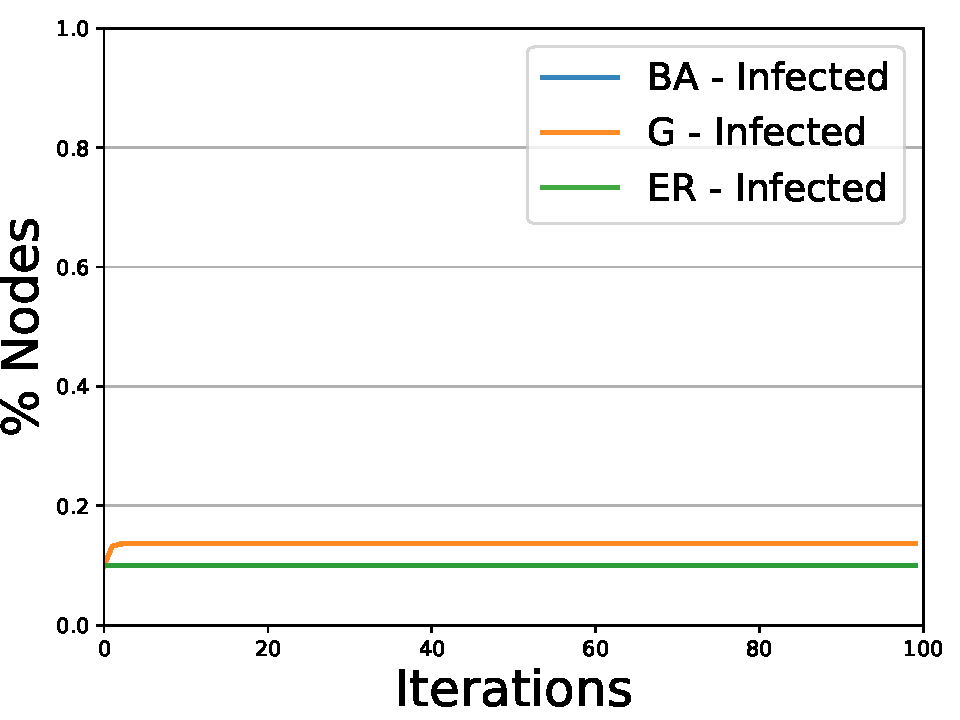
\includegraphics{images/spreading/threshold/trend_comparison_disfree.pdf}
            }
            \caption{Disease-free state with higher threshold, $\tau=0.2$ }
          \end{subfigure}
          \caption{Threshold model applied to the networks, the Barabasi trend is superimposed by the Erdos-Renyi one.}
      \label{diff_thr_total}
  \end{figure}


      




% section threshold_model (end)


\section{The New York Times vs La Repubblica vs Sputnik Italia}

Let's assume that the same news it is initially spread by 3 different sources, with very different degree values:
\begin{itemize}
\item The New York Times, the biggest hub,  with in-degree $k_{in}=19064$  and \#followers=41595294.
\item La Repubblica, with $k_{in}=961$ and \#followers=2843075.
\item Sputnik Italia, with $k_{in}=71$ and \#followers=6490.  
\end{itemize}
We applied the SIR model obtaining two scenarios, a viral news reaching a large part of the network and a minor news vanishing 
out after a mildly spread. The scenarios depicted in Fig. \ref{fig:viral_news} have been obtained maintaining the same transmission rate $\beta$ and changing the recovery rate $\mu$.
In the viral news scenario the different degree values caused only a modest translation in time of the spread trends, with the same percentages
of infected nodes. This result may be explained clearly by the properties of the free-scale networks: the presence of the hubs and the ultra small world property cause a fast spreading from @sputnik\_italia to the hubs, who infect immediately a large fraction of the network.
In the second scenario, by decreasing the $\lambda$ ratio below a certain threshold, the news spread by @sputnik\_italia nodes probably did not reach the hubs and the infection did not propagate.

The two presented scenarios can explain the fact that for example \textit{fake news} can also begin spreading from peripheral, small nodes and propagates virally over a network. The difference between the two scenarios is carried by the intrinsic transmission properties of the news,
independently from the properties of the carrier: the message it is more important than the messenger.

   \begin{figure}[H]
        \centering
        \begin{subfigure}{0.45\textwidth}
            \resizebox{\textwidth}{!}{
                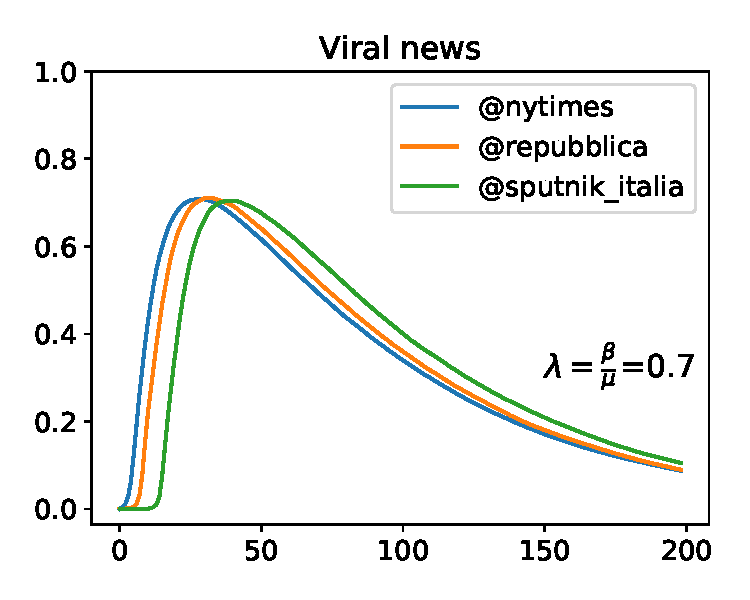
\includegraphics{images/spreading/news_viral.pdf}
            }
            \caption{}
            \label{diff_thr}
        \end{subfigure}
        \begin{subfigure}{0.45\textwidth}
            \resizebox{\textwidth}{!}{
                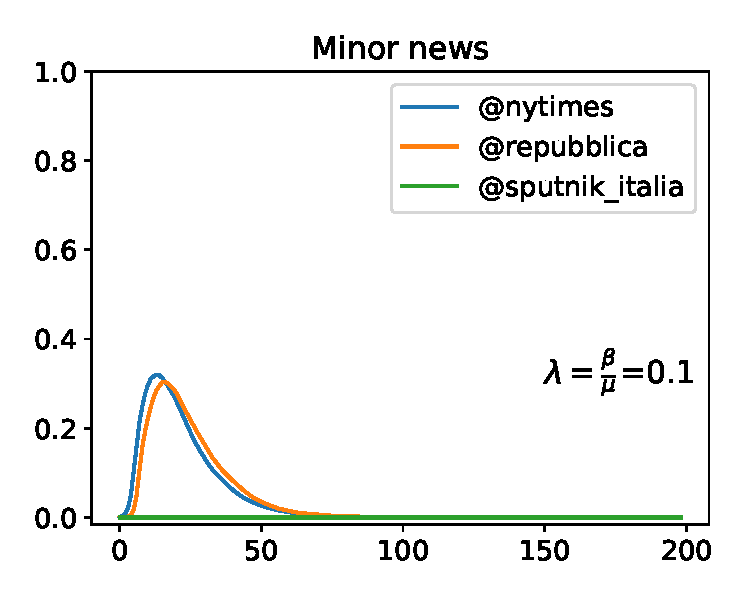
\includegraphics{images/spreading/news_minor.pdf}
            }
            \caption{}
            \label{diff_thr_er}
          \end{subfigure}
          \caption{Viral news spreading: infected percentages trends.}
          \label{fig:viral_news}
\end{figure}


    
% chapter spreading (end)
